\chapter{SUNDIALS Package Installation Procedure}\label{c:install}

The installation of any {\sundials} package is accomplished by installing the
{\sundials} suite as a whole, according to the instructions that
follow. The same procedure applies whether or not the downloaded
file contains one or all solvers in {\sundials}.

The {\sundials} suite (or individual solvers) are distributed as
compressed archives (\id{.tar.gz}). The name of the distribution
archive is of the form {\em solver}\id{-x.y.z.tar.gz}, where {\em solver}
is one of: \id{sundials}, \id{cvode}, \id{cvodes}, \id{arkode}, \id{ida},
\id{idas}, or \id{kinsol}, and \id{x.y.z} represents the version number
(of the {\sundials} suite or of the individual solver).
%%
To begin the installation, first uncompress and expand the sources, by issuing
\begin{verbatim}
   % tar xzf solver-x.y.z.tar.gz
\end{verbatim}
This will extract source files under a directory {\em solver}\id{-x.y.z}.

Starting with version \id{2.6.0} of {\sundials}, CMake is the only supported method
of installation.
The explanations of the installation procedure begins with a few common observations:
%%
\begin{itemize}

\item The remainder of this chapter will follow these conventions:
  \begin{description}
  \item[{\em solverdir}]
    is the directory {\em solver}\id{-x.y.z} created above; i.e., the
    directory containing the {\sundials} sources.
  \item[{\em builddir}]
    is the (temporary) directory under which {\sundials} is built.
  \item[{\em instdir}]
    is the directory under which the {\sundials} exported header files
    and libraries will be installed. Typically, header files are exported under a directory
    {\em instdir}\id{/include} while libraries are installed under {\em instdir}\id{/CMAKE\_INSTALL\_LIBDIR},
    with {\em instdir} and\\
    \id{CMAKE\_INSTALL\_LIBDIR} specified at configuration time.
  \end{description}

\item For {\sundials} CMake-based installation, in-source builds are prohibited; in other words, the
  build directory {\em builddir} can {\bf not} be the same as {\em solverdir}
  and such an attempt will lead to an error. This
  prevents ``polluting'' the source tree and allows efficient builds
  for different configurations and/or options.

\item {\warn}The installation directory {\em instdir} can {\bf not} be the same as
  the source directory {\em solverdir}.

\item By default, only the libraries and header files are exported to the installation
  directory {\em instdir}.  If enabled by the user (with the
  appropriate toggle for CMake), the
  examples distributed with {\sundials} will be built together with
  the solver libraries but the installation step will result in
  exporting (by default in a subdirectory of the installation
  directory) the example sources and sample outputs together with
  automatically generated configuration files that reference the {\em
  installed} {\sundials} headers and libraries.  As such, these
  configuration files for the {\sundials} examples can be used as
  ``templates'' for your own problems. CMake installs \id{CMakeLists.txt} files and also
  (as an option available only under Unix/Linux) \id{Makefile} files. Note this
  installation approach also allows the option of building the
  {\sundials} examples without having to install them.  (This can be
  used as a sanity check for the freshly built libraries.)

\item Even if generation of shared libraries is enabled, only static libraries
  are created for the FCMIX modules.  (Because of the use of fixed names for
  the Fortran user-provided subroutines, FCMIX shared libraries would result in
  ``undefined symbol'' errors at link time.)

\end{itemize}


%%===============================================================================
\section{CMake-based installation}\label{s:cmake_inst}
%%===============================================================================

CMake-based installation provides a platform-independent build system. CMake can generate
Unix and Linux Makefiles, as well as KDevelop, Visual Studio, and
(Apple) XCode project files from the same configuration file.
In addition, CMake also provides a GUI front end and which allows an interactive build and
installation process.

The {\sundials} build process requires CMake version \id{3.1.3} or
higher and a working {\CC} compiler.  On Unix-like operating systems, it
also requires Make (and \id{curses}, including its development libraries,
for the GUI front end to CMake, \id{ccmake}), while on Windows it
requires Visual Studio. CMake is continually adding new features, and
the latest version can be downloaded from {\tt http://www.cmake.org}. Build instructions for CMake
(only necessary for Unix-like systems) can be found on the CMake website.
Once CMake is installed, Linux/Unix users will be able to use \id{ccmake},
while Windows users will be able to use \id{CMakeSetup}.

As previously noted, when using CMake to configure, build and install {\sundials}, it is always
required to use a separate build directory. While in-source builds are possible, they are
explicitly prohibited by the {\sundials} CMake scripts (one of the reasons being that, unlike
autotools, CMake does not provide a \id{make distclean} procedure and it is therefore
difficult to clean-up the source tree after an in-source build). By ensuring a separate build
directory, it is an easy task for the user to clean-up all traces of the build by simply removing
the build directory. CMake does generate a \id{make clean} which will remove files generated by the
compiler and linker.

\subsection{Configuring, building, and installing on Unix-like systems}

The default CMake configuration will build all included solvers and
associated examples and will build static and shared libraries. The
{\em instdir} defaults to \id{/usr/local} and can be changed by
setting the \id{CMAKE\_INSTALL\_PREFIX} variable.  Support for FORTRAN
and all other options are disabled.

CMake can be used from the command line with the \id{cmake} command, or from a \id{curses}-based GUI
by using the \id{ccmake} command. Examples for using both methods will be presented.
For the examples shown it is assumed that there is a top level {\sundials} directory
with appropriate source, build and install directories:

\begin{verbatim}
   % mkdir (...)sundials/instdir
   % mkdir (...)sundials/builddir
   % cd (...)sundials/builddir
\end{verbatim}

%%
%% Building with the GUI configuration
%%
\subsubsection*{Building with the GUI}

Using CMake with the GUI follows this general process:
\begin{itemize}
\item Select and modify values, run configure (\id{c} key)
\item New values are denoted with an asterisk
\item To set a variable, move the cursor to the variable and press enter
  \begin{itemize}
  \item If it is a boolean (ON/OFF) it will toggle the value
  \item If it is string or file, it will allow editing of the string
  \item For file and directories, the \id{<tab>} key can be used to complete
  \end{itemize}
\item Repeat until all values are set as desired and the generate option is available (\id{g} key)
\item Some variables (advanced variables) are not visible right away
\item To see advanced variables, toggle to advanced mode (\id{t} key)
\item To search for a variable press \id{/} key, and to repeat the search, press the
\id{n} key
\end{itemize}

To build the default configuration using the GUI, from the {\em builddir} enter
the ccmake command and point to the {\em solverdir}:

\begin{verbatim}
    % ccmake ../solverdir
\end{verbatim}

The default configuration screen is shown in Figure
\ref{f:ccmakedefault}.
\begin{figure}[!ht]
{\centerline{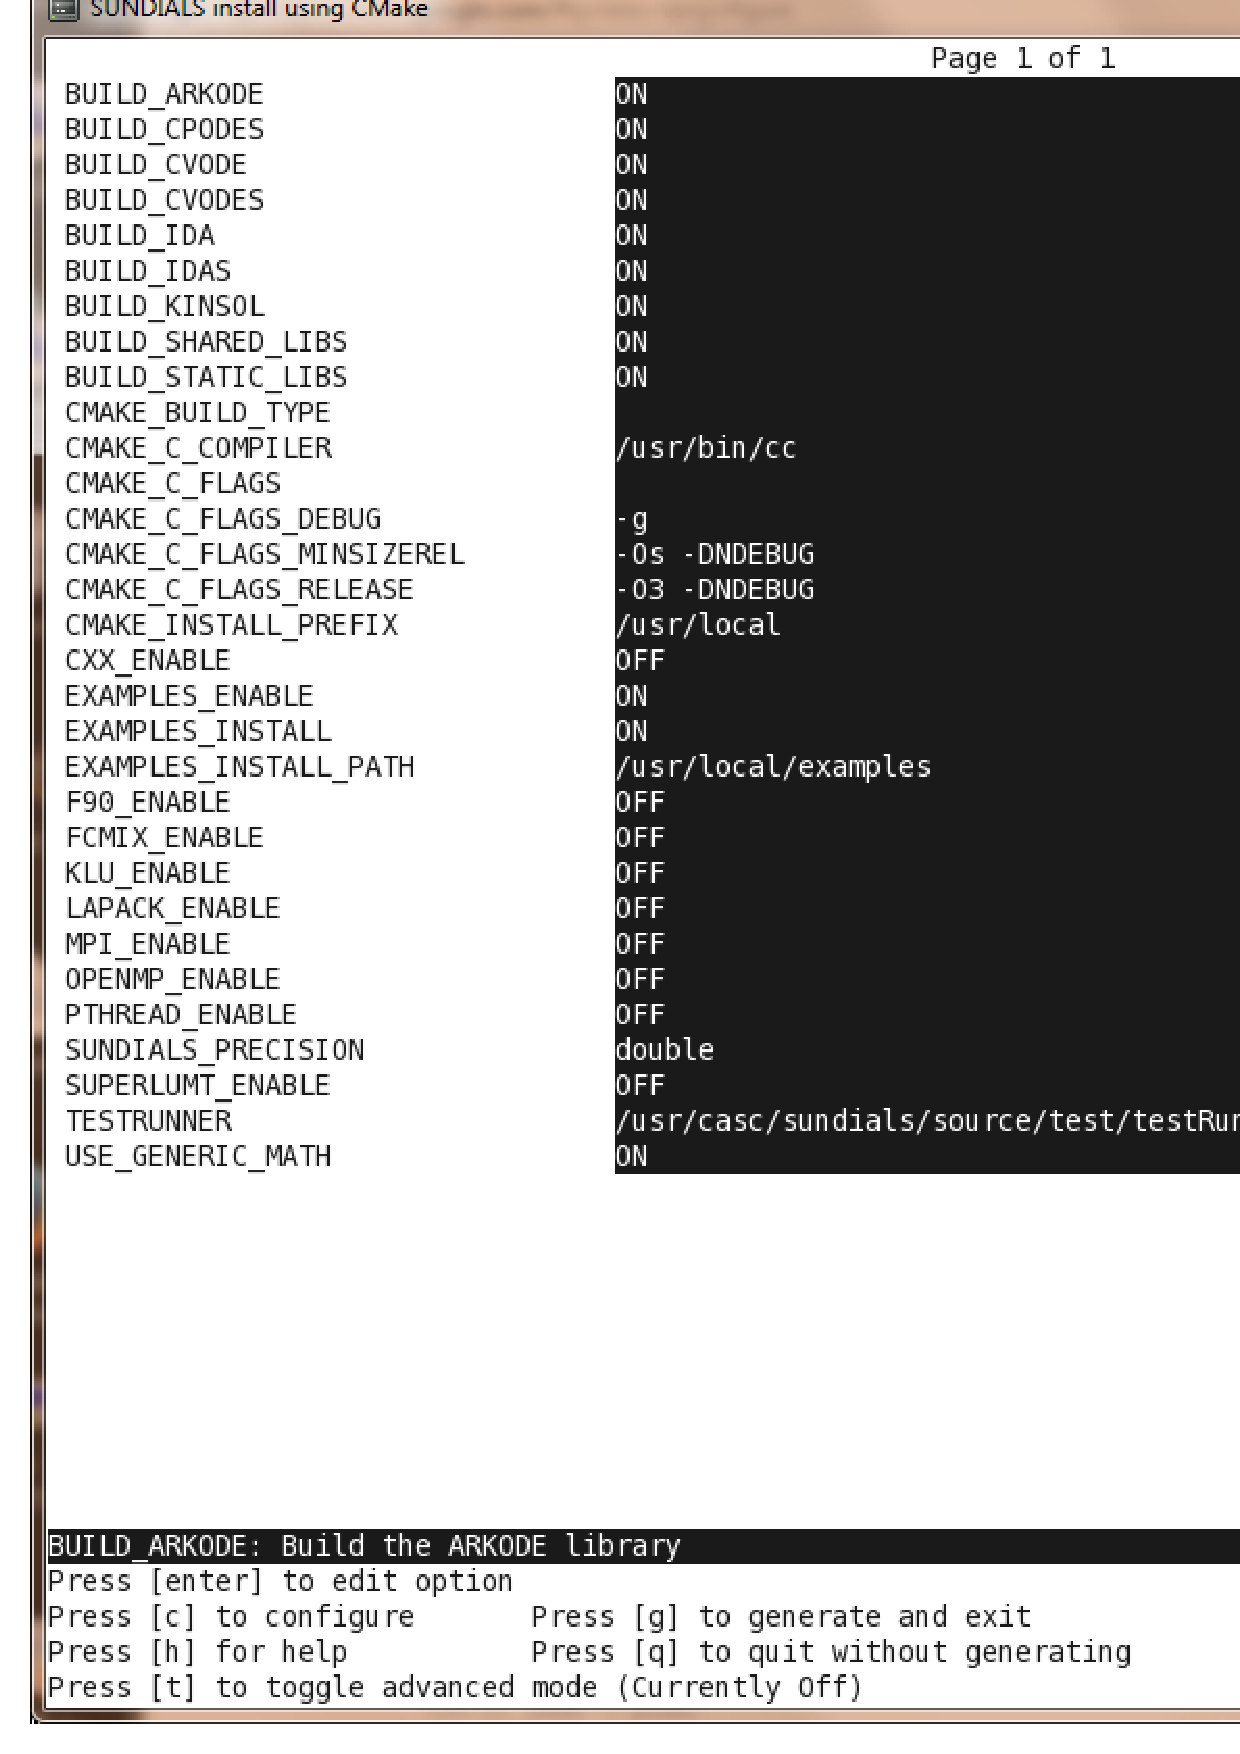
\includegraphics[width=\textwidth]{ccmakedefault}}}
\caption [Initial {\em ccmake} configuration screen]
{Default configuration screen. Note: Initial screen is empty.
To get this default configuration, press 'c' repeatedly (accepting default values denoted with asterisk)
until the 'g' option is available.}
\label{f:ccmakedefault}
\end{figure}

The default {\em instdir} for both {\sundials} and corresponding examples
can be changed by setting the \id{CMAKE\_INSTALL\_PREFIX} and
the \id{EXAMPLES\_INSTALL\_PATH} as shown in figure
\ref{f:ccmakeprefix}.
\begin{figure}[!ht]
{\centerline{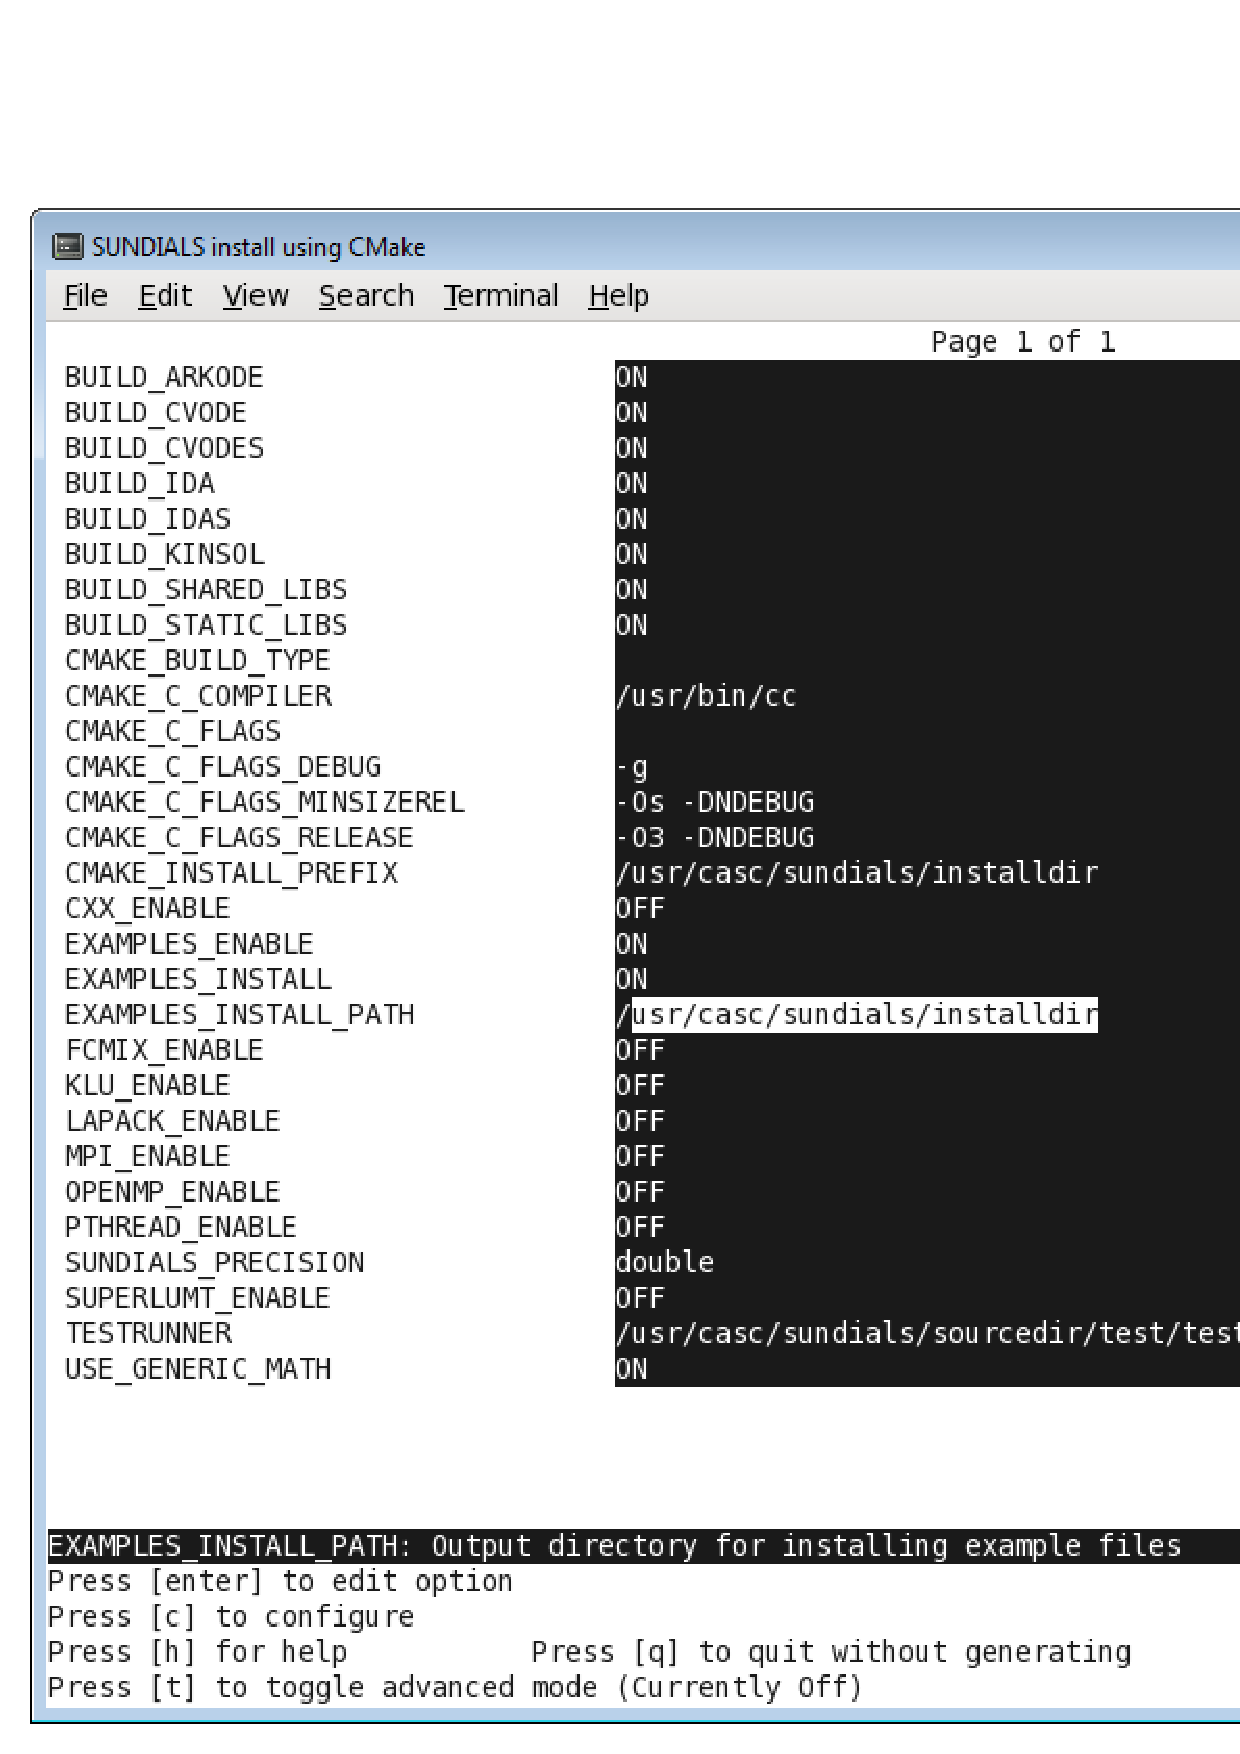
\includegraphics[width=\textwidth]{ccmakeprefix}}}
\caption [Changing the {\em instdir}]
{Changing the {\em instdir} for {\sundials} and
corresponding {\id examples} }
\label{f:ccmakeprefix}
\end{figure}

Pressing the (\id{g} key) will generate makefiles including all dependencies
and all rules to build {\sundials} on this system.
Back at the command prompt, you can now run:

\begin{verbatim}
  % make
\end{verbatim}

To install {\sundials} in the installation directory specified in the configuration, simply run:

\begin{verbatim}
  % make install
\end{verbatim}

%%
%% *** NOTE: The TestRunner will not be distributed at this time.
%% *** Thus the following is commented out from the documentation.
%% TestRunner
%%
%\subsubsection*{Testing Installation}
%The distribution of {\sundials} includes several examples corresponding to the solvers to be
%installed. Also included in the source bundle is a test script: \id{testRunner}, configured by CMake
%to test the included examples.
%To run the tests, enter:

%\begin{verbatim}
%  % make test
%\end{verbatim}
%The output of \id{testRunner} should look similar to the screens in figure
%\ref{f:testrunner}. The success of each test is based on a line-by-line comparison of expected output files, bundled with the source code, with
%the output of the newly compiled examples. The file compare does allow some differences in rounding for float values.\\\\
%NOTE: Some tests may {\em fail} due to differences in machine architecture, compiler versions, third party libraries etc.{\warn}

%\begin{figure}[!ht]
%{\centerline{\includegraphics{figure=testrunnertop.eps,width=\textwidth}}}
%\vspace{3 mm}
%{\centerline{\includegraphics{figure=testrunnerbot.eps,width=\textwidth}}}
%\caption [Running {\em testRunner}]
%{Invoking {\em testRunner} with {\id make test} to execute all configured
%{\id examples} }
%\label{f:testrunner}
%\end{figure}


%%
%% Building from the command line
%%
\subsubsection*{Building from the command line}

Using CMake from the command line is simply a matter of specifying CMake variable settings
with the \id{cmake} command.  The following will build the default configuration:

\begin{verbatim}
   % cmake -DCMAKE_INSTALL_PREFIX=/home/myname/sundials/instdir \
   > -DEXAMPLES_INSTALL_PATH=/home/myname/sundials/instdir/examples \
   > ../solverdir
   % make
   % make install
\end{verbatim}


\subsection{Configuration options (Unix/Linux)}\label{ss:configuration_options_nix}

A complete list of all available options for a CMake-based {\sundials}
configuration is provide below. Note that the default values shown are for
a typical configuration on a Linux system and are provided as illustration only.

\begin{description}
\item[\id{BLAS\_ENABLE}] -
  Enable BLAS support
  \\
  Default: OFF
  \\
  Note: Setting this option to ON will trigger additional CMake
  options. See additional information on building with BLAS enabled
  in \ref{ss:externallibs}.
\item[\id{BLAS\_LIBRARIES}] -
  BLAS library
  \\
  Default: /usr/lib/libblas.so
  \\
  Note: CMake will search for libraries in your \id{LD\_LIBRARY\_PATH} prior
  to searching default system paths.
\item[\id{BUILD\_ARKODE}] -
  Build the ARKODE library
  \\
  Default: ON
\item[\id{BUILD\_CVODE}] -
  Build the CVODE library
  \\
  Default: ON
\item[\id{BUILD\_CVODES}] -
  Build the CVODES library
  \\
  Default: ON
\item[\id{BUILD\_IDA}] -
   Build the IDA library
  \\
   Default: ON
\item[\id{BUILD\_IDAS}] -
  Build the IDAS library
  \\
  Default: ON
\item[\id{BUILD\_KINSOL}] -
  Build the KINSOL library
  \\
  Default: ON
\item[\id{BUILD\_SHARED\_LIBS}] -
  Build shared libraries
  \\
  Default: ON
\item[\id{BUILD\_STATIC\_LIBS}] -
  Build static libraries
  \\
  Default: ON
\item[\id{CMAKE\_BUILD\_TYPE}] -
  Choose the type of build, options are:
  \id{None} (CMAKE\_C\_FLAGS used), \id{Debug}, \id{Release},
  \id{RelWithDebInfo}, and \id{MinSizeRel}
  \\
  Default:
  \\
  Note: Specifying a build type will trigger the corresponding
  build type specific compiler flag options below which will be
  appended to the flags set by
  CMAKE\_{\textless}language{\textgreater}\_FLAGS.
\item[\id{CMAKE\_C\_COMPILER}] -
  C compiler
  \\
  Default: /usr/bin/cc
\item[\id{CMAKE\_C\_FLAGS}] -
  Flags for C compiler
  \\
  Default:
\item[\id{CMAKE\_C\_FLAGS\_DEBUG}] -
  Flags used by the C compiler during debug builds
  \\
  Default: -g
\item[\id{CMAKE\_C\_FLAGS\_MINSIZEREL}] -
  Flags used by the C compiler during release minsize builds
  \\
  Default: -Os -DNDEBUG
\item[\id{CMAKE\_C\_FLAGS\_RELEASE}] -
  Flags used by the C compiler during release builds
  \\
  Default: -O3 -DNDEBUG
\item[\id{CMAKE\_CXX\_COMPILER}] -
  {\CPP} compiler
  \\
  Default: /usr/bin/c++
  \\
  Note: A {\CPP} compiler (and all related options) are only
  triggered if {\CPP} examples are enabled (\id{EXAMPLES\_ENABLE\_CXX}
  is ON). All {\sundials} solvers can be used from {\CPP} applications
  by default without setting any additional configuration options.
\item[\id{CMAKE\_CXX\_FLAGS}] -
  Flags for {\CPP} compiler
  \\
  Default:
\item[\id{CMAKE\_CXX\_FLAGS\_DEBUG}] -
  Flags used by the {\CPP} compiler during debug builds
  \\
  Default: -g
\item[\id{CMAKE\_CXX\_FLAGS\_MINSIZEREL}] -
  Flags used by the {\CPP} compiler during release minsize builds
  \\
  Default: -Os -DNDEBUG
\item[\id{CMAKE\_CXX\_FLAGS\_RELEASE}] -
  Flags used by the {\CPP} compiler during release builds
  \\
  Default: -O3 -DNDEBUG
\item[\id{CMAKE\_Fortran\_COMPILER}] -
  Fortran compiler
  \\
  Default: /usr/bin/gfortran
  \\
  Note: Fortran support (and all related options) are triggered only if
  either Fortran-C support is enabled (\id{FCMIX\_ENABLE} is ON) or
  BLAS/LAPACK support is enabled (\id{BLAS\_ENABLE} or \id{LAPACK\_ENABLE} is ON).
\item[\id{CMAKE\_Fortran\_FLAGS}] -
  Flags for Fortran compiler
  \\
  Default:
\item[\id{CMAKE\_Fortran\_FLAGS\_DEBUG}] -
  Flags used by the Fortran compiler during debug builds
  \\
  Default: -g
\item[\id{CMAKE\_Fortran\_FLAGS\_MINSIZEREL}] -
  Flags used by the Fortran compiler during release minsize builds
  \\
  Default: -Os
\item[\id{CMAKE\_Fortran\_FLAGS\_RELEASE}] -
  Flags used by the Fortran compiler during release builds
  \\
  Default: -O3
\item[\id{CMAKE\_INSTALL\_PREFIX}] -
  Install path prefix, prepended onto install directories
  \\
  Default: /usr/local
  \\
  Note: The user must have write access to the location specified through
  this option. Exported {\sundials} header files and libraries will be
  installed under subdirectories \id{include} and
  \id{CMAKE\_INSTALL\_LIBDIR} of \id{CMAKE\_INSTALL\_PREFIX}, respectively.
\item[\id{CMAKE\_INSTALL\_LIBDIR}] -
  Library installation directory
  \\
  Default:
  \\
  Note: This is the directory within \id{CMAKE\_INSTALL\_PREFIX} that the {\sundials}
  libraries will be installed under. The default is automatically set based on the
  operating system using the GNUInstallDirs CMake module.
\item[\id{Fortran\_INSTALL\_MODDIR}] -
  Fortran module installation directory
  \\
  Default: fortran
\item[\id{CUDA\_ENABLE}] -
  Build the {\sundials} {\cuda} vector module.
  \\
  Default: OFF
\item[\id{EXAMPLES\_ENABLE\_C}] -
  Build the {\sundials} {\CC} examples
  \\
  Default: ON
\item[\id{EXAMPLES\_ENABLE\_CUDA}] -
  Build the {\sundials} {\cuda} examples
  \\
  Default: OFF
  \\
  Note: You need to enable {\cuda} support to build these examples.
\item[\id{EXAMPLES\_ENABLE\_CXX}] -
  Build the {\sundials} {\CPP} examples
  \\
  Default: OFF unless \id{Trilinos\_ENABLE} is ON.
\item[\id{EXAMPLES\_ENABLE\_F77}] -
  Build the {\sundials} Fortran77 examples
  \\
  Default: ON (if \id{F77\_INTERFACE\_ENABLE} is ON)
\item[\id{EXAMPLES\_ENABLE\_F90}] -
  Build the {\sundials} Fortran90 examples
  \\
  Default: ON (if \id{F77\_INTERFACE\_ENABLE} is ON)
\item[\id{EXAMPLES\_ENABLE\_F2003}] -
  Build the {\sundials} Fortran2003 examples
  \\
  Default: ON (if \id{F2003\_INTERFACE\_ENABLE} is ON)
\item[\id{EXAMPLES\_INSTALL}] -
  Install example files
  \\
  Default: ON
  \\
  Note: This option is triggered when any of the {\sundials}
  example programs are enabled \\
  (\id{EXAMPLES\_ENABLE\_$<$language$>$} is ON). If the user requires
  installation of example programs then the sources and sample output files
  for all {\sundials} modules that are currently enabled will be exported to
  the directory specified by \id{EXAMPLES\_INSTALL\_PATH}. A CMake configuration
  script will also be automatically generated and exported to the same directory.
  Additionally, if the configuration is done under a Unix-like system, makefiles
  for the compilation of the example programs (using the installed {\sundials} libraries)
  will be automatically generated and exported to the directory
  specified by \id{EXAMPLES\_INSTALL\_PATH}.
\item[\id{EXAMPLES\_INSTALL\_PATH}] -
  Output directory for installing example files
  \\
  Default: /usr/local/examples
  \\
  Note: The actual default value for this option will be an \id{examples}
  subdirectory created under \id{CMAKE\_INSTALL\_PREFIX}.
\item[\id{F77\_INTERFACE\_ENABLE}] -
  Enable Fortran-C support via the Fortran 77 interfaces
  \\
  Default: OFF
\item[\id{F2003\_INTERFACE\_ENABLE}] -
  Enable Fortran-C support via the Fortran 2003 interfaces
  \\
  Default: OFF
\item[\id{HYPRE\_ENABLE}] -
  Enable {\hypre} support
  \\
  Default: OFF
  \\
  Note: See additional information on building with {\hypre} enabled in
  \ref{ss:externallibs}.
\item[\id{HYPRE\_INCLUDE\_DIR}] -
  Path to {\hypre} header files
\item[\id{HYPRE\_LIBRARY\_DIR}] -
  Path to {\hypre} installed library files
\item[\id{KLU\_ENABLE}] -
  Enable KLU support
  \\
  Default: OFF
  \\
  Note: See additional information on building with KLU enabled in
  \ref{ss:externallibs}.
\item[\id{KLU\_INCLUDE\_DIR}] -
  Path to SuiteSparse header files
\item[\id{KLU\_LIBRARY\_DIR}] -
  Path to SuiteSparse installed library files
\item[\id{LAPACK\_ENABLE}] -
  Enable LAPACK support
  \\
  Default: OFF
  \\
  Note: Setting this option to ON will trigger additional CMake
  options. See additional information on building with LAPACK enabled
  in \ref{ss:externallibs}.
\item[\id{LAPACK\_LIBRARIES}] -
  LAPACK (and BLAS) libraries
  \\
  Default: /usr/lib/liblapack.so;/usr/lib/libblas.so
  \\
  Note: CMake will search for libraries in your \id{LD\_LIBRARY\_PATH} prior
  to searching default system paths.
\item[\id{MPI\_ENABLE}] -
  Enable MPI support. This will build the parallel {\nvector} and the
  MPI-aware version of the ManyVector library.
  \\
  Default: OFF
  \\
  Note: Setting this option to ON will trigger several additional options
  related to MPI.
\item[\id{MPI\_C\_COMPILER}] -
  \id{mpicc} program
  \\
  Default:
\item[\id{MPI\_CXX\_COMPILER}] -
  \id{mpicxx} program
  \\
  Default:
  \\
  Note: This option is triggered only if MPI is enabled
  (\id{MPI\_ENABLE} is ON) and {\CPP} examples are enabled
  (\id{EXAMPLES\_ENABLE\_CXX} is ON). All {\sundials}
  solvers can be used from {\CPP} MPI applications by default
  without setting any additional configuration options other than
  \id{MPI\_ENABLE}.
\item[\id{MPI\_Fortran\_COMPILER}] -
  \id{mpif77} or \id{mpif90} program
  \\
  Default:
  \\
  Note: This option is triggered only if MPI is enabled
  (\id{MPI\_ENABLE} is ON) and Fortran-C support is enabled
  (\id{F77\_INTERFACE\_ENABLE} or \id{F2003\_INTERFACE\_ENABLE} is ON).
\item[\id{MPIEXEC\_EXECUTABLE}] -
  Specify the executable for running MPI programs
  \\
  Default: \id{mpirun}
  \\
  Note: This option is triggered only if MPI is enabled
  (\id{MPI\_ENABLE} is ON).
  %% \\
  %% Note: This can either be set to \id{mpirun} for OpenMPI or \id{srun} if jobs are
  %% managed by \id{SLURM} - Simple Linux Utility for Resource Management as exists on
  %% LLNL's high performance computing clusters.
\item[\id{OPENMP\_ENABLE}] -
  Enable {\openmp} support (build the {\openmp} {\nvector}).
  \\
  Default: OFF
\item[\id{OPENMP\_DEVICE\_ENABLE}] -
  Enable {\openmp} device offloading (build the OpenMPDEV nvector) if supported by
  the provided compiler.
  \\
  Default: OFF
\item[\id{SKIP\_OPENMP\_DEVICE\_CHECK}] - \textbf{advanced option} -
  Skip the check done to see if the {\openmp} provided by the compiler
  supports {\openmp} device offloading.
  \\
  Default: OFF
\item[\id{PETSC\_ENABLE}] -
  Enable {\petsc} support
  \\
  Default: OFF
  \\
  Note: See additional information on building with {\petsc} enabled
  in \ref{ss:externallibs}.
\item[\id{PETSC\_INCLUDE\_DIR}] -
  Path to {\petsc} header files
\item[\id{PETSC\_LIBRARY\_DIR}] -
  Path to {\petsc} installed library files
\item[\id{PTHREAD\_ENABLE}] -
  Enable Pthreads support (build the Pthreads {\nvector}).
  \\
  Default: OFF
\item[\id{RAJA\_ENABLE}] -
  Enable {\raja} support (build the {\raja} {\nvector}).
  \\
  Default: OFF
  \\
  Note: You need to enable {\cuda} in order to build the {\raja} vector module.
\item[\id{SUNDIALS\_F77\_FUNC\_CASE}] - \textbf{advanced option} -
  Specify the case to use in the Fortran name-mangling scheme, options
  are: \id{lower} or \id{upper}
  \\
  Default:
  \\
  Note: The build system will attempt to infer the Fortran
  name-mangling scheme using the Fortran compiler. This option should
  only be used if a Fortran compiler is not available or to override
  the inferred or default (\id{lower}) scheme if one can not be
  determined. If used, \id{SUNDIALS\_F77\_FUNC\_UNDERSCORES} must also
  be set.
\item[\id{SUNDIALS\_F77\_FUNC\_UNDERSCORES}] - \textbf{advanced option} -
  Specify the number of underscores to append in the Fortran
  name-mangling scheme, options are: \id{none}, \id{one}, or \id{two}
  \\
  Default:
  \\
  Note: The build system will attempt to infer the Fortran
  name-mangling scheme using the Fortran compiler. This option should
  only be used if a Fortran compiler is not available or to override
  the inferred or default (\id{one}) scheme if one can not be
  determined. If used, \id{SUNDIALS\_F77\_FUNC\_CASE} must also be set.
\item[\id{SUNDIALS\_INDEX\_TYPE}] - \textbf{advanced option} -
  Integer type used for {\sundials} indices. The size must match the size provided for
  the \\ \noindent \id{SUNDIALS\_INDEX\_SIZE} option.
  \\
  Default:
  \\
  Note:
  In past SUNDIALS versions, a user could set this option to \id{INT64\_T} to use 64-bit
  integers, or \id{INT32\_T} to use 32-bit integers. Starting in SUNDIALS 3.2.0, these
  special values are deprecated. For SUNDIALS 3.2.0 and up, a user will only need to use
  the \id{SUNDIALS\_INDEX\_SIZE} option in most cases.
\item[\id{SUNDIALS\_INDEX\_SIZE}] -
  Integer size (in bits) used for indices in {\sundials}, options are: \id{32} or \id{64}
  \\
  Default: \id{64}
  \\
  Note:
  The build system tries to find an integer type of appropriate size. Candidate 64-bit
  integer types are (in order of preference): \id{int64\_t}, \id{\_\_int64}, \id{long long}, and \id{long}.
  Candidate 32-bit integers are (in order of preference): \id{int32\_t}, \id{int}, and \id{long}.
  The advanced option, \id{SUNDIALS\_INDEX\_TYPE} can be used to provide a type not listed here.
\item[\id{SUNDIALS\_PRECISION}] -
  Precision used in {\sundials}, options are: \id{double}, \id{single}, or \id{extended}
  \\
  Default: \id{double}
\item[\id{SUPERLUDIST\_ENABLE}] -
  Enable {\superludist} support
  \\
  Default: OFF
  \\
  Note: See additional information on building with {\superludist} enabled
  in \ref{ss:externallibs}.
\item[\id{SUPERLUDIST\_INCLUDE\_DIR}] -
  Path to {\superludist} header files (typically SRC directory)
\item[\id{SUPERLUDIST\_LIBRARY\_DIR}] -
  Path to {\superludist} installed library files
\item[\id{SUPERLUDIST\_LIBRARIES}] -
  Semi-colon separated list of libraries needed for {\superludist}
\item[\id{SUPERLUDIST\_OpenMP}] -
  Enable {\sundials} support for {\superludist} built with {\openmp}
  \\
  Default: OFF
  \\
  Note: {\superludist} must be built with {\openmp} support for this option to function
  properly. Additionally the environment variable \id{OMP\_NUM\_THREADS} must be set to
  the desired number of threads.
\item[\id{SUPERLUMT\_ENABLE}] -
  Enable {\superlumt} support
  \\
  Default: OFF
  \\
  Note: See additional information on building with {\superlumt} enabled
  in \ref{ss:externallibs}.
\item[\id{SUPERLUMT\_INCLUDE\_DIR}] -
  Path to SuperLU\_MT header files (typically SRC directory)
\item[\id{SUPERLUMT\_LIBRARY\_DIR}] -
  Path to SuperLU\_MT installed library files
\item[\id{SUPERLUMT\_THREAD\_TYPE}] -
  Must be set to Pthread or {\openmp}
  \\
  Default: Pthread
\item[\id{Trilinos\_ENABLE}] -
  Enable {\trilinos} support (build the {\tpetra} {\nvector}).
  \\
  Default: OFF
\item[\id{Trilinos\_DIR}] -
  Path to the Trilinos install directory.
  \\
  Default:
\item[\id{TRILINOS\_INTERFACE\_C\_COMPILER}] - \textbf{advanced option} -
  Set the {\CC} compiler for building the {\trilinos} interface
  (i.e., {\nvectrilinos} and the examples that use it).
  \\
  Default: The {\CC} compiler exported from the found {\trilinos} installation
  if \id{USE\_XSDK\_DEFAULTS=OFF}. \id{CMAKE\_C\_COMPILER} or \id{MPI\_C\_COMPILER} if \id{USE\_XSDK\_DEFAULTS=ON}.
  \\
  Note: It is recommended to use the same compiler that was used to build the {\trilinos} library.
\item[\id{TRILINOS\_INTERFACE\_C\_COMPILER\_FLAGS}] - \textbf{advanced option} -
  Set the {\CC} compiler flags for {\trilinos} interface
  (i.e., {\nvectrilinos} and the examples that use it).
  \\
  Default: The {\CC} compiler flags exported from the found {\trilinos} installation
  if \id{USE\_XSDK\_DEFAULTS=OFF}. \id{CMAKE\_C\_FLAGS} if \id{USE\_XSDK\_DEFAULTS=ON}.
  \\
  Note: It is recommended to use the same flags that were used to build the {\trilinos} library.
\item[\id{TRILINOS\_INTERFACE\_CXX\_COMPILER}] - \textbf{advanced option} -
  Set the {\CPP} compiler for builing {\trilinos} interface
  (i.e., {\nvectrilinos} and the examples that use it).
  \\
  Default: The {\CPP} compiler exported from the found {\trilinos} installation
  if \id{USE\_XSDK\_DEFAULTS=OFF}. \id{CMAKE\_CXX\_COMPILER} or \id{MPI\_CXX\_COMPILER} if \id{USE\_XSDK\_DEFAULTS=ON}.
  \\
  Note: It is recommended to use the same compiler that was used to build the {\trilinos} library.
\item[\id{TRILINOS\_INTERFACE\_CXX\_COMPILER\_FLAGS}] - \textbf{advanced option} -
  Set the {\CPP} compiler flags for {\trilinos} interface
  (i.e., {\nvectrilinos} and the examples that use it).
  \\
  Default: The {\CPP} compiler flags exported from the found {\trilinos} installation
  if \id{USE\_XSDK\_DEFAULTS=OFF}. \id{CMAKE\_CXX\_FLAGS} if \id{USE\_XSDK\_DEFAULTS=ON}.
  \\
  Note: Is is recommended to use the same flags that were used to build the {\trilinos} library.
\item[\id{USE\_GENERIC\_MATH}] -
  Use generic (stdc) math libraries
  \\
  Default: ON



\end{description}

\subsubsection*{xSDK Configuration Options}

{\sundials} supports CMake configuration options defined by the
Extreme-scale Scientific Software Development Kit (xSDK) community
policies (see {\tt https://xsdk.info} for more information). xSDK
CMake options are unused by default but may be activated by setting
\id{USE\_XSDK\_DEFAULTS} to ON.

{\warn} When xSDK options are active, they will overwrite the
corresponding {\sundials} option and may have different default values
(see details below). As such the equivalent {\sundials} options should
not be used when configuring with xSDK options. In the GUI front end
to CMake (\id{ccmake}), setting \id{USE\_XSDK\_DEFAULTS} to ON will
hide the corresponding {\sundials} options as advanced CMake variables.
During configuration, messages are output detailing
which xSDK flags are active and the equivalent {\sundials} options
that are replaced. Below is a complete list xSDK options and the
corresponding {\sundials} options if applicable.

\begin{description}
\item[\id{TPL\_BLAS\_LIBRARIES}] -
  BLAS library
  \\
  Default: /usr/lib/libblas.so
  \\
  {\sundials} equivalent: \id{BLAS\_LIBRARIES}
  \\
  Note: CMake will search for libraries in your \id{LD\_LIBRARY\_PATH} prior
  to searching default system paths.
\item[\id{TPL\_ENABLE\_BLAS}] -
  Enable BLAS support
  \\
  Default: OFF
  \\
  {\sundials} equivalent: \id{BLAS\_ENABLE}
\item[\id{TPL\_ENABLE\_HYPRE}] -
  Enable {\hypre} support
  \\
  Default: OFF
  \\
  {\sundials} equivalent: \id{HYPRE\_ENABLE}
\item[\id{TPL\_ENABLE\_KLU}] -
  Enable KLU support
  \\
  Default: OFF
  \\
  {\sundials} equivalent: \id{KLU\_ENABLE}
\item[\id{TPL\_ENABLE\_PETSC}] -
  Enable {\petsc} support
  \\
  Default: OFF
  \\
  {\sundials} equivalent: \id{PETSC\_ENABLE}
\item[\id{TPL\_ENABLE\_LAPACK}] -
  Enable LAPACK support
  \\
  Default: OFF
  \\
  {\sundials} equivalent: \id{LAPACK\_ENABLE}
\item[\id{TPL\_ENABLE\_SUPERLUDIST}] -
  Enable {\superludist} support
  \\
  Default: OFF
  \\
  {\sundials} equivalent: \id{SUPERLUDIST\_ENABLE}
\item[\id{TPL\_ENABLE\_SUPERLUMT}] -
  Enable SuperLU\_MT support
  \\
  Default: OFF
  \\
  {\sundials} equivalent: \id{SUPERLUMT\_ENABLE}
\item[\id{TPL\_HYPRE\_INCLUDE\_DIRS}] -
  Path to {\hypre} header files
  \\
  {\sundials} equivalent: \id{HYPRE\_INCLUDE\_DIR}
\item[\id{TPL\_HYPRE\_LIBRARIES}] -
  {\hypre} library
  \\
  {\sundials} equivalent: N/A
\item[\id{TPL\_KLU\_INCLUDE\_DIRS}] -
  Path to KLU header files
  \\
  {\sundials} equivalent: \id{KLU\_INCLUDE\_DIR}
\item[\id{TPL\_KLU\_LIBRARIES}] -
  KLU library
  \\
  {\sundials} equivalent: N/A
\item[\id{TPL\_LAPACK\_LIBRARIES}] -
  LAPACK (and BLAS) libraries
  \\
  Default: /usr/lib/liblapack.so;/usr/lib/libblas.so
  \\
  {\sundials} equivalent: \id{LAPACK\_LIBRARIES}
  \\
  Note: CMake will search for libraries in your \id{LD\_LIBRARY\_PATH} prior
  to searching default system paths.
\item[\id{TPL\_PETSC\_INCLUDE\_DIRS}] -
  Path to {\petsc} header files
  \\
  {\sundials} equivalent: \id{PETSC\_INCLUDE\_DIR}
\item[\id{TPL\_PETSC\_LIBRARIES}] -
  {\petsc} library
  \\
  {\sundials} equivalent: N/A
\item[\id{TPL\_SUPERLUDIST\_INCLUDE\_DIRS}] -
  Path to {\superludist} header files
  \\
  {\sundials} equivalent: \id{SUPERLUDIST\_INCLUDE\_DIR}
\item[\id{TPL\_SUPERLUDIST\_LIBRARIES}] -
  Semi-colon separated list of libraries needed for {\superludist}
  including the {\superludist} library itself
  \\
  {\sundials} equivalent: \id{SUPERLUDIST\_LIBRARIES}
\item[\id{TPL\_SUPERLUDIST\_OPENMP}] -
  Enable {\sundials} support for {\superludist} built with {\openmp}
  \\
  {\sundials} equivalent: \id{SUPERLUDIST\_OPENMP}
\item[\id{TPL\_SUPERLUMT\_LIBRARIES}] -
  SuperLU\_MT library
  \\
  {\sundials} equivalent: N/A
\item[\id{TPL\_SUPERLUMT\_THREAD\_TYPE}] -
  SuperLU\_MT library thread type
  \\
  {\sundials} equivalent: \id{SUPERLUMT\_THREAD\_TYPE}
\item[\id{USE\_XSDK\_DEFAULTS}] -
  Enable xSDK default configuration settings
  \\
  Default: OFF
  \\
  {\sundials} equivalent: N/A
  \\
  Note: Enabling xSDK defaults also sets \id{CMAKE\_BUILD\_TYPE} to \id{Debug}
\item[\id{XSDK\_ENABLE\_FORTRAN}] -
  Enable {\sundials} Fortran interfaces
  \\
  Default: OFF
  \\
  {\sundials} equivalent: \id{F77\_INTERFACE\_ENABLE}/\id{F2003\_INTERFACE\_ENABLE}
\item[\id{XSDK\_INDEX\_SIZE}] -
  Integer size (bits) used for indices in {\sundials}, options are: \id{32} or \id{64}
  \\
  Default: \id{32}
  \\
  {\sundials} equivalent: \id{SUNDIALS\_INDEX\_SIZE}
\item[\id{XSDK\_PRECISION}] -
  Precision used in {\sundials}, options are: \id{double}, \id{single}, or \id{quad}
  \\
  Default: \id{double}
  \\
  {\sundials} equivalent: \id{SUNDIALS\_PRECISION}
\end{description}



%%===============================================================================

\subsection{Configuration examples}

The following examples will help demonstrate usage of the CMake configure options.

\noindent To configure {\sundials} using the default C and Fortran compilers,
and default \id{mpicc} and \id{mpif77} parallel compilers,
enable compilation of examples, and install libraries, headers, and
example sources under subdirectories of
\id{/home/myname/sundials/}, use:

\begin{verbatim}
   % cmake \
   > -DCMAKE_INSTALL_PREFIX=/home/myname/sundials/instdir \
   > -DEXAMPLES_INSTALL_PATH=/home/myname/sundials/instdir/examples \
   > -DMPI_ENABLE=ON \
   > -DFCMIX_ENABLE=ON \
   > /home/myname/sundials/solverdir
   %
   % make install
   %
\end{verbatim}

\noindent To disable installation of the examples, use:
\begin{verbatim}
   % cmake \
   > -DCMAKE_INSTALL_PREFIX=/home/myname/sundials/instdir \
   > -DEXAMPLES_INSTALL_PATH=/home/myname/sundials/instdir/examples \
   > -DMPI_ENABLE=ON \
   > -DFCMIX_ENABLE=ON \
   > -DEXAMPLES_INSTALL=OFF \
   > /home/myname/sundials/solverdir
   %
   % make install
   %
\end{verbatim}

%%===============================================================================
\subsection{Working with external Libraries} \label{ss:externallibs}

The {\sundials} suite contains many options to enable implementation flexibility
when developing solutions. The following are some notes addressing specific configurations
when using the supported third party libraries.
When building {\sundials} as a shared library external libraries any
used with {\sundials} must also be build as a shared library or as a
static library compiled with the \id{-fPIC} flag.{\warn}

\subsubsection*{Building with BLAS}
{\sundials} does not utilize BLAS directly but it may be needed by other
external libraries that {\sundials} can be built with (e.g. LAPACK,
{\petsc}, SuperLU\_MT, etc.). To enable BLAS, set the \id{BLAS\_ENABLE}
option to \id{ON}. If the directory containing the BLAS library is in
the \id{LD\_LIBRARY\_PATH} environment variable, CMake will set the
\id{BLAS\_LIBRARIES} variable accordingly, otherwise CMake will
attempt to find the BLAS library in standard system locations. To
explicitly tell CMake what libraries to use, the \id{BLAS\_LIBRARIES}
variable can be set to the desired library. Example:
\begin{verbatim}
   % cmake \
   > -DCMAKE_INSTALL_PREFIX=/home/myname/sundials/instdir \
   > -DEXAMPLES_INSTALL_PATH=/home/myname/sundials/instdir/examples \
   > -DBLAS_ENABLE=ON \
   > -DBLAS_LIBRARIES=/myblaspath/lib/libblas.so \
   > -DSUPERLUMT_ENABLE=ON \
   > -DSUPERLUMT_INCLUDE_DIR=/mysuperlumtpath/SRC
   > -DSUPERLUMT_LIBRARY_DIR=/mysuperlumtpath/lib
   > /home/myname/sundials/solverdir
   %
   % make install
   %
\end{verbatim}
{\warn}When allowing CMake to automatically locate the LAPACK library,
CMake \textit{may} also locate the corresponding BLAS library.

If a working Fortran compiler is not available to infer the Fortran
name-mangling scheme, the options \id{SUNDIALS\_F77\_FUNC\_CASE} and
\id{SUNDIALS\_F77\_FUNC\_UNDERSCORES} \textit{must} be set in order to
bypass the check for a Fortran compiler and define the name-mangling
scheme. The defaults for these options in earlier versions of
{\sundials} were \id{lower} and \id{one} respectively.


\subsubsection*{Building with LAPACK}
To enable LAPACK, set the \id{LAPACK\_ENABLE} option to \id{ON}.
If the directory containing the LAPACK library is in the
\id{LD\_LIBRARY\_PATH} environment variable, CMake will set the
\id{LAPACK\_LIBRARIES} variable accordingly, otherwise CMake will
attempt to find the LAPACK library in standard system locations. To
explicitly tell CMake what library to use, the \id{LAPACK\_LIBRARIES}
variable can be set to the desired libraries. {\warn}When setting
the LAPACK location explicitly the location of the corresponding BLAS
library will also need to be set. Example:
\begin{verbatim}
   % cmake \
   > -DCMAKE_INSTALL_PREFIX=/home/myname/sundials/instdir \
   > -DEXAMPLES_INSTALL_PATH=/home/myname/sundials/instdir/examples \
   > -DBLAS_ENABLE=ON \
   > -DBLAS_LIBRARIES=/mylapackpath/lib/libblas.so \
   > -DLAPACK_ENABLE=ON \
   > -DLAPACK_LIBRARIES=/mylapackpath/lib/liblapack.so \
   > /home/myname/sundials/solverdir
   %
   % make install
   %
\end{verbatim}
{\warn}When allowing CMake to automatically locate the LAPACK library,
CMake \textit{may} also locate the corresponding BLAS library.

If a working Fortran compiler is not available to infer the Fortran
name-mangling scheme, the options \id{SUNDIALS\_F77\_FUNC\_CASE} and
\id{SUNDIALS\_F77\_FUNC\_UNDERSCORES} \textit{must} be set in order to
bypass the check for a Fortran compiler and define the name-mangling
scheme. The defaults for these options in earlier versions of
{\sundials} were \id{lower} and \id{one} respectively.

\subsubsection*{Building with KLU}
The KLU libraries are part of SuiteSparse, a suite of sparse matrix software,
available from the Texas A\&M University website: {\tt http://faculty.cse.tamu.edu/davis/suitesparse.html}.
{\sundials} has been tested with SuiteSparse version 5.3.0.
To enable KLU, set \id{KLU\_ENABLE} to \id{ON}, set \id{KLU\_INCLUDE\_DIR} to the \id{include}
path of the KLU installation and set \id{KLU\_LIBRARY\_DIR} to the \id{lib} path of the KLU installation.
The CMake configure will result in populating the following variables: \id{AMD\_LIBRARY},
\id{AMD\_LIBRARY\_DIR}, \id{BTF\_LIBRARY}, \id{BTF\_LIBRARY\_DIR},
\id{COLAMD\_LIBRARY}, \id{COLAMD\_LIBRARY\_DIR}, and
\newline\id{KLU\_LIBRARY}.

\subsubsection*{Building with SuperLU\_MT}
The SuperLU\_MT libraries are available for download from the Lawrence Berkeley National Laboratory website:
{\tt http://crd-legacy.lbl.gov/$\sim$xiaoye/SuperLU/\#superlu\_mt}.
{\sundials} has been tested with SuperLU\_MT version 3.1.
To enable SuperLU\_MT, set  \id{SUPERLUMT\_ENABLE} to \id{ON}, set \id{SUPERLUMT\_INCLUDE\_DIR}
to the \id{SRC} path of the SuperLU\_MT installation, and set the variable
\newline\id{SUPERLUMT\_LIBRARY\_DIR} to the \id{lib} path of the SuperLU\_MT installation.
At the same time, the variable
\id{SUPERLUMT\_THREAD\_TYPE} must be set to either \id{Pthread} or \id{{\openmp}}.

\noindent Do not mix thread types when building {\sundials} solvers.
If threading is enabled for {\sundials} by having either \id{OPENMP\_ENABLE} or \id{PTHREAD\_ENABLE} set to \id{ON}
then SuperLU\_MT should be set to use the same threading type.{\warn}

\subsubsection*{Building with {\superludist}}
The {\superludist} libraries are available for download from the Lawrence Berkeley National Laboratory website:
{\tt http://crd-legacy.lbl.gov/$\sim$xiaoye/SuperLU/\#superlu\_dist}.
{\sundials} has been tested with {\superludist} greater than 6.1.
To enable {\superludist}, set \id{SUPERLUDIST\_ENABLE} to \id{ON}, set \id{SUPERLUDIST\_INCLUDE\_DIR}
to the include directory of the {\superludist} installation (typically \id{SRC}), and set the variable
\newline\id{SUPERLUDIST\_LIBRARY\_DIR} to the path to library directory of the {\superludist} installation (typically \id{lib}). At the same time, the variable
\id{SUPERLUDIST\_LIBRARIES} must be set to a semi-colon separated list of
other libraries {\superludist} depends on. For example, if {\superludist} was
built with LAPACK, then include the LAPACK library in this list.
If {\superludist} was built with {\openmp} support, then you may set \id{SUPERLUDIST\_OPENMP}
to \id{ON} to utilize the {\openmp} functionality of {\superludist}.

\noindent Do not mix thread types when building {\sundials} solvers.
If threading is enabled for {\sundials} by having \id{PTHREAD\_ENABLE} set to \id{ON}
then {\superludist} should not be set to use {\openmp}.{\warn}

\subsubsection*{Building with PETSc}
The {\petsc} libraries are available for download from the Argonne National Laboratory website:
{\tt http://www.mcs.anl.gov/petsc}.
{\sundials} has been tested with {\petsc} version 3.10.3.
To enable {\petsc}, set  \id{PETSC\_ENABLE} to \id{ON}, set \id{PETSC\_INCLUDE\_DIR}
to the \id{include} path of the {\petsc} installation, and set the variable
\id{PETSC\_LIBRARY\_DIR} to the \id{lib} path of the {\petsc} installation.


\subsubsection*{Building with {\hypre}}
The {\hypre} libraries are available for download from the Lawrence Livermore
National Laboratory website: {\tt http://computation.llnl.gov/projects/hypre}.
%{\tt http://computation.llnl.gov/projects/hypre-scalable-linear-solvers-multigrid-methods}.
{\sundials} has been tested with {\hypre} version 2.14.0.
To enable {\hypre}, set  \id{HYPRE\_ENABLE} to \id{ON}, set \id{HYPRE\_INCLUDE\_DIR}
to the \id{include} path of the {\hypre} installation, and set the variable
\id{HYPRE\_LIBRARY\_DIR} to the \id{lib} path of the {\hypre} installation.

\subsubsection*{Building with CUDA}
{\sundials} {\cuda} modules and examples have been tested with version 9.0 of the
{\cuda} toolkit. To build them, you need to install the Toolkit and compatible
NVIDIA drivers. Both are available for download from the NVIDIA website:
{\tt https://developer.nvidia.com/cuda-downloads}. To enable {\cuda},
set \id{CUDA\_ENABLE} to \id{ON}. If {\cuda} is installed in a
nonstandard location, you may be prompted to set the variable
\id{CUDA\_TOOLKIT\_ROOT\_DIR} with your {\cuda} Toolkit installation
path. To enable {\cuda} examples, set \id{EXAMPLES\_ENABLE\_CUDA} to \id{ON}.

\subsubsection*{Building with RAJA}
{\raja} is a performance portability layer developed by Lawrence
Livermore National Laboratory and can be obtained from {\tt https://github.com/LLNL/RAJA}.
{\sundials} {\raja} modules and examples have been tested with {\raja}
version 0.6. Building {\sundials} {\raja} modules requires a
{\cuda}-enabled {\raja} installation. To enable {\raja}, set
\id{CUDA\_ENABLE} and \id{RAJA\_ENABLE} to \id{ON}. If {\raja} is
installed in a nonstandard location you will be prompted to set the
variable \id{RAJA\_DIR} with the path to the {\raja} CMake
configuration file. To enable building the {\raja} examples set
\id{EXAMPLES\_ENABLE\_CUDA} to \id{ON}.

\subsubsection*{Building with Trilinos}
{\trilinos} is a suite of numerical libraries developed by Sandia National
Laboratories. It can be obtained at {\tt https://github.com/trilinos/Trilinos}.
{\sundials} {\trilinos} modules and examples have been tested with {\trilinos}
version 12.14. To enable {\trilinos}, set
\id{Trilinos\_ENABLE} to \id{ON}. If {\trilinos} is
installed in a nonstandard location you will be prompted to set the
variable \id{Trilinos\_DIR} with the path to the {\trilinos} CMake
configuration file. It is desireable to build the {\trilinos} vector interface
with same compiler and options that were used to build {\trilinos}.
CMake will try to find the correct compiler settings automatically from the
{\trilinos} configuration file. If that is not successful,
the compilers and options can be manually set with the following CMake variables:
\begin{itemize}
\item
\id{Trilinos\_INTERFACE\_C\_COMPILER}
\item
\id{Trilinos\_INTERFACE\_C\_COMPILER\_FLAGS}
\item
\id{Trilinos\_INTERFACE\_CXX\_COMPILER}
\item
\id{Trilinos\_INTERFACE\_CXX\_COMPILER\_FLAGS}
\end{itemize}

\subsection{Testing the build and installation}

If {\sundials} was configured with
\id{EXAMPLES\_ENABLE\_$<$language$>$} options to \id{ON}, then a set of
regression tests can be run after building with the \id{make} command
by running:
\begin{verbatim}
  % make test
\end{verbatim}
Additionally, if \id{EXAMPLES\_INSTALL} was also set to \id{ON}, then
a set of smoke tests can be run after installing with the \id{make install}
command by running:
\begin{verbatim}
  % make test_install
\end{verbatim}

%%===============================================================================
\section{Building and Running Examples}
%%===============================================================================
Each of the {\sundials} solvers is distributed with a set of examples
demonstrating basic usage. To build and install the examples, set at
least of the \id{EXAMPLES\_ENABLE\_$<$language$>$} options to \id{ON}, and
set \id{EXAMPLES\_INSTALL} to \id{ON}.
Specify the installation path for the examples with the variable \id{EXAMPLES\_INSTALL\_PATH}. CMake will generate
\id{CMakeLists.txt} configuration files (and \id{Makefile} files if on Linux/Unix) that reference the
{\em installed} {\sundials} headers and libraries.

Either the \id{CMakeLists.txt} file or the traditional \id{Makefile} may be used to build the examples
as well as serve as a template for creating user developed solutions.
To use the supplied \id{Makefile} simply run \id{make} to compile and generate the executables.
To use CMake from within the installed example directory, run \id{cmake} (or \id{ccmake} to use the GUI)
followed by \id{make} to compile the example code.
Note that if CMake is used, it will overwrite the traditional \id{Makefile} with a new CMake-generated \id{Makefile}.
The resulting output from running the examples can be compared with example output bundled
in the {\sundials} distribution.

\noindent NOTE: There will potentially be differences in the output due to machine architecture, compiler versions,
use of third party libraries etc.{\warn}


%%===============================================================================
\section{Configuring, building, and installing  on Windows}\label{s:cmake_windows}
%%===============================================================================
CMake can also be used to build {\sundials} on Windows. To build {\sundials} for
use with Visual Studio the following steps should be performed:
\begin{enumerate}
\item Unzip the downloaded tar file(s) into a directory. This will be the {\em solverdir}
\item Create a separate {\em builddir}
\item Open a Visual Studio Command Prompt and cd to {\em builddir}
\item Run cmake-gui ../{\em solverdir}
\begin{enumerate}
\item Hit Configure
\item Check/Uncheck solvers to be built
\item Change CMAKE\_INSTALL\_PREFIX to {\em instdir}
\item Set other options as desired
\item Hit Generate
\end{enumerate}
\item Back in the VS Command Window:
\begin{enumerate}
\item Run msbuild ALL\_BUILD.vcxproj
\item Run msbuild INSTALL.vcxproj
\end{enumerate}
\end{enumerate}

\noindent The resulting libraries will be in the {\em instdir}.
\noindent The {\sundials} project can also now be opened in Visual Studio.
Double click on the ALL\_BUILD.vcxproj file to open the project.
Build the whole {\em solution} to create the {\sundials} libraries.
To use the {\sundials} libraries in your own projects, you must
set the include directories for your project,
add the {\sundials} libraries to your project solution,
and set the {\sundials} libraries as dependencies for your project.

%%===============================================================================
\section{Installed libraries and exported header files}
%%===============================================================================

Using the CMake {\sundials} build system, the command
\begin{verbatim}
   % make install
\end{verbatim}
will install the libraries under {\em libdir} and the public header
files under {\em includedir}. The values for these directories are
{\em instdir}\id{/CMAKE\_INSTALL\_LIBDIR} and {\em instdir}\id{/include},
respectively. The location can be changed by setting the CMake variable \id{CMAKE\_INSTALL\_PREFIX}.
Although all installed libraries reside under {\em libdir}\id{/CMAKE\_INSTALL\_LIBDIR}, the public
header files are further organized into subdirectories under {\em includedir}\id{/include}.

The installed libraries and exported header files are listed for
reference in Table \ref{t:sundials_files}.
The file extension .{\em lib}
is typically \id{.so} for shared libraries and \id{.a} for static libraries.
Note that, in the Tables, names are relative to {\em libdir}
for libraries and to {\em includedir} for header files.

A typical user program need not explicitly include any of the shared
{\sundials} header files from under the {\em includedir}\id{/include}\id{/sundials}
directory since they are explicitly included by the appropriate solver
header files ({\em e.g.}, \id{cvode\_dense.h} includes
\id{sundials\_dense.h}). However, it is both legal and safe to do so,
and would be useful, for example, if the functions declared in \id{sundials\_dense.h}
are to be used in building a preconditioner.

%---------------------------------------------------------------------------
% Table of installed files
%---------------------------------------------------------------------------

\newlength{\colLenOne}
\settowidth{\colLenOne}{{\sunnonlinsolfixedpoint}}

\newlength{\colLenTwo}
\settowidth{\colLenTwo}{Header files}

\newlength{\colLenThree}
\setlength{\colLenThree}{\textwidth}
\addtolength{\colLenThree}{-0.5in}
\addtolength{\colLenThree}{-\colLenOne}
\addtolength{\colLenThree}{-\colLenTwo}

%\caption{{\sundials} libraries and header files (cont.)}\label{t:sundials_files2}

\clearpage
\tablecaption{{\sundials} libraries and header files}\label{t:sundials_files}
\tablefirsthead{\hline}
\tablehead{\hline \multicolumn{4}{|l|}{\small\slshape continued from last page} \\
           \hline}
\tabletail{\hline \multicolumn{4}{|r|}{\small\slshape continued on next page} \\ \hline}
\begin{xtabular}{|p{\colLenOne}|p{\colLenTwo}|p{0.5\colLenThree} p{0.5\colLenThree}|}

%% --------------------------------------------------
{\shared}
 & Libraries    & n/a  & \\
\cline{2-4}
& Header files & sundials/sundials\_config.h                         &                           \\
&              & sundials/sundials\_fconfig.h                        &                           \\
&              & sundials/sundials\_types.h                          &                           \\
&              & sundials/sundials\_math.h                           &                           \\
&              & sundials/sundials\_nvector.h                        &                           \\
&              & sundials/sundials\_fnvector.h                       &                           \\
&              & sundials/sundials\_matrix.h                         &                           \\
&              & sundials/sundials\_linearsolver.h                   &                           \\
&              & sundials/sundials\_iterative.h                      &                           \\
&              & sundials/sundials\_direct.h                         &                           \\
&              & sundials/sundials\_dense.h                          &                           \\
&              & sundials/sundials\_band.h                           &                           \\
&              & sundials/sundials\_nonlinearsolver.h                &                           \\
&              & sundials/sundials\_version.h                        &                           \\
&              & sundials/sundials\_mpi\_types.h                     &                           \\
\hline
%% --------------------------------------------------
{\nvecs}
& Libraries    & libsundials\_nvecserial.{\em lib}                   &                           \\
&              & libsundials\_fnvecserial\_mod.{\em lib}             &                           \\
&              & libsundials\_fnvecserial.a                          &                           \\
\cline{2-4}
& Header files & nvector/nvector\_serial.h                           &                           \\
\cline{2-4}
& Module files & fnvector\_serial\_mod.mod                           &                           \\
\hline
%% --------------------------------------------------
{\nvecp}
& Libraries    & libsundials\_nvecparallel.{\em lib}                 &                           \\
&              & libsundials\_fnvecparallel.a                        &                           \\
&              & libsundials\_fnvecparallel\_mod.{\em lib}           &                           \\
\cline{2-4}
& Header files & nvector/nvector\_parallel.h                         &                           \\
\cline{2-4}
& Module files & fnvector\_parallel\_mod.mod                         &                           \\
\hline
%% --------------------------------------------------
{\nvecmanyvector}
& Libraries    & libsundials\_nvecmanyvector.{\em lib}               &                           \\
\cline{2-4}
& Header files & nvector/nvector\_manyvector.h                       &                           \\
\hline
%% --------------------------------------------------
{\nvecmpimanyvector}
& Libraries    & libsundials\_nvecmpimanyvector.{\em lib}            &                           \\
\cline{2-4}
& Header files & nvector/nvector\_mpimanyvector.h                    &                           \\
\hline
%% --------------------------------------------------
{\nvecmpiplusx}
& Libraries    & libsundials\_nvecmpiplusx.{\em lib}                 &                           \\
\cline{2-4}
& Header files & nvector/nvector\_mpiplusx.h                         &                           \\
\hline
%% --------------------------------------------------
{\nvecopenmp}
& Libraries    & libsundials\_nvecopenmp.{\em lib}                   &                           \\
&              & libsundials\_fnvecopenmp\_mod.{\em lib}             &                           \\
&              & libsundials\_fnvecopenmp.a                          &                           \\
\cline{2-4}
& Header files & nvector/nvector\_openmp.h                           &                           \\
\cline{2-4}
& Module files & fnvector\_openmp\_mod.mod                           &                           \\
\hline
%% --------------------------------------------------
{\nvecopenmpdev}
& Libraries    & libsundials\_nvecopenmpdev.{\em lib}                &                           \\
\cline{2-4}
& Header files & nvector/nvector\_openmpdev.h                        &                           \\
\hline
%% --------------------------------------------------
{\nvecpthreads}
& Libraries    & libsundials\_nvecpthreads.{\em lib}                 &                           \\
&              & libsundials\_fnvecpthreads\_mod.{\em lib}           &                           \\
&              & libsundials\_fnvecpthreads.a                        &                           \\
\cline{2-4}
& Header files & nvector/nvector\_pthreads.h                         &                           \\
\cline{2-4}
& Module files & fnvector\_pthreads\_mod.mod                         &                           \\
\hline
%% --------------------------------------------------
{\nvecph}
& Libraries    & libsundials\_nvecparhyp.{\em lib}                   &                           \\
\cline{2-4}
& Header files & nvector/nvector\_parhyp.h                           &                           \\
\hline
%% --------------------------------------------------
{\nvecpetsc}
& Libraries    & libsundials\_nvecpetsc.{\em lib}                    &                           \\
\cline{2-4}
& Header files & nvector/nvector\_petsc.h                            &                           \\
\hline
%% --------------------------------------------------
{\nveccuda}
& Libraries    & libsundials\_nveccuda.{\em lib}                     &                           \\
\cline{2-4}
& Header files & nvector/nvector\_cuda.h                             &                           \\
&              & nvector/cuda/ThreadPartitioning.hpp                 &                           \\
&              & nvector/cuda/Vector.hpp                             &                           \\
&              & nvector/cuda/VectorKernels.cuh                      &                           \\
\hline
%% --------------------------------------------------
{\nvecraja}
& Libraries    & libsundials\_nveccudaraja.{\em lib}                 &                           \\
\cline{2-4}
& Header files & nvector/nvector\_raja.h                             &                           \\
&              & nvector/raja/Vector.hpp                             &                           \\
\hline
%% --------------------------------------------------
{\nvectrilinos}
& Libraries    & libsundials\_nvectrilinos.{\em lib}                 &                           \\
\cline{2-4}
& Header files & nvector/nvector\_trilinos.h                         &                           \\
&              & nvector/trilinos/SundialsTpetraVectorInterface.hpp  &                           \\
&              & nvector/trilinos/SundialsTpetraVectorKernels.hpp    &                           \\
\hline
%% --------------------------------------------------
{\sunmatband}
& Libraries    & libsundials\_sunmatrixband.{\em lib}                &                           \\
&              & libsundials\_fsunmatrixband\_mod.{\em lib}          &                           \\
&              & libsundials\_fsunmatrixband.a                       &                           \\
\cline{2-4}
& Header files & sunmatrix/sunmatrix\_band.h                         &                           \\
\cline{2-4}
& Module files & fsunmatrix\_band\_mod.mod                           &                           \\
\hline
%% --------------------------------------------------
{\sunmatdense}
& Libraries    & libsundials\_sunmatrixdense.{\em lib}               &                           \\
&              & libsundials\_fsunmatrixdense\_mod.{\em lib}         &                           \\
&              & libsundials\_fsunmatrixdense.a                      &                           \\
\cline{2-4}
& Header files & sunmatrix/sunmatrix\_dense.h                        &                           \\
\cline{2-4}
& Module files & fsunmatrix\_dense\_mod.mod                          &                           \\
\hline
%% --------------------------------------------------
{\sunmatsparse}
& Libraries    & libsundials\_sunmatrixsparse.{\em lib}              &                           \\
&              & libsundials\_fsunmatrixsparse\_mod.{\em lib}        &                           \\
&              & libsundials\_fsunmatrixsparse.a                     &                           \\
\cline{2-4}
& Header files & sunmatrix/sunmatrix\_sparse.h                       &                           \\
\cline{2-4}
& Module files & fsunmatrix\_sparse\_mod.mod                         &                           \\
\hline
%% --------------------------------------------------
{\sunmatslunrloc}
& Libraries    & libsundials\_sunmatrixslunrloc.{\em lib}            &                           \\
\cline{2-4}
& Header files & sunmatrix/sunmatrix\_slunrloc.h                     &                           \\
\hline
%% --------------------------------------------------
{\sunlinsolband}
& Libraries    & libsundials\_sunlinsolband.{\em lib}                &                           \\
&              & libsundials\_fsunlinsolband\_mod.{\em lib}          &                           \\
&              & libsundials\_fsunlinsolband.a                       &                           \\
\cline{2-4}
& Header files & sunlinsol/sunlinsol\_band.h                         &                           \\
\cline{2-4}
& Module files & fsunlinsol\_band\_mod.mod                           &                           \\
\hline
%% --------------------------------------------------
{\sunlinsoldense}
& Libraries    & libsundials\_sunlinsoldense.{\em lib}               &                           \\
&              & libsundials\_fsunlinsoldense\_mod.{\em lib}         &                           \\
&              & libsundials\_fsunlinsoldense.a                      &                           \\
\cline{2-4}
& Header files & sunlinsol/sunlinsol\_dense.h                        &                           \\
\cline{2-4}
& Module files & fsunlinsol\_dense\_mod.mod                          &                           \\
\hline
%% --------------------------------------------------
{\sunlinsolklu}
& Libraries    & libsundials\_sunlinsolklu.{\em lib}                 &                           \\
&              & libsundials\_fsunlinsolklu\_mod.{\em lib}           &                           \\
&              & libsundials\_fsunlinsolklu.a                        &                           \\
\cline{2-4}
& Header files & sunlinsol/sunlinsol\_klu.h                          &                           \\
\cline{2-4}
& Module files & fsunlinsol\_klu\_mod.mod                            &                           \\
\hline
%% --------------------------------------------------
{\sunlinsollapband}
& Libraries    & libsundials\_sunlinsollapackband.{\em lib}          &                           \\
&              & libsundials\_fsunlinsollapackband.a                 &                           \\
\cline{2-4}
& Header files & sunlinsol/sunlinsol\_lapackband.h                   &                           \\
\hline
%% --------------------------------------------------
{\sunlinsollapdense}
& Libraries    & libsundials\_sunlinsollapackdense.{\em lib}         &                           \\
&              & libsundials\_fsunlinsollapackdense.a                &                           \\
\cline{2-4}
& Header files & sunlinsol/sunlinsol\_lapackdense.h                  &                           \\
\hline
%% --------------------------------------------------
{\sunlinsolpcg}
& Libraries    & libsundials\_sunlinsolpcg.{\em lib}                 &                           \\
&              & libsundials\_fsunlinsolpcg\_mod.{\em lib}           &                           \\
&              & libsundials\_fsunlinsolpcg.a                        &                           \\
\cline{2-4}
& Header files & sunlinsol/sunlinsol\_pcg.h                          &                           \\
\cline{2-4}
& Module files & fsunlinsol\_pcg\_mod.mod                            &                           \\
\hline
%% --------------------------------------------------
{\sunlinsolspbcgs}
& Libraries    & libsundials\_sunlinsolspbcgs.{\em lib}              &                           \\
&              & libsundials\_fsunlinsolspbcgs\_mod.{\em lib}        &                           \\
&              & libsundials\_fsunlinsolspbcgs.a                     &                           \\
\cline{2-4}
& Header files & sunlinsol/sunlinsol\_spbcgs.h                       &                           \\
\cline{2-4}
& Module files & fsunlinsol\_spbcgs\_mod.mod                         &                           \\
\hline
%% --------------------------------------------------
{\sunlinsolspfgmr}
& Libraries    & libsundials\_sunlinsolspfgmr.{\em lib}              &                           \\
&              & libsundials\_fsunlinsolspfgmr\_mod.{\em lib}        &                           \\
&              & libsundials\_fsunlinsolspfgmr.a                     &                           \\
\cline{2-4}
& Header files & sunlinsol/sunlinsol\_spfgmr.h                       &                           \\
\cline{2-4}
& Module files & fsunlinsol\_spfgmr\_mod.mod                         &                           \\
\hline
%% --------------------------------------------------
{\sunlinsolspgmr}
& Libraries    & libsundials\_sunlinsolspgmr.{\em lib}               &                           \\
&              & libsundials\_fsunlinsolspgmr\_mod.{\em lib}         &                           \\
&              & libsundials\_fsunlinsolspgmr.a                      &                           \\
\cline{2-4}
& Header files & sunlinsol/sunlinsol\_spgmr.h                        &                           \\
\cline{2-4}
& Module files & fsunlinsol\_spgmr\_mod.mod                          &                           \\
\hline
%% --------------------------------------------------
{\sunlinsolsptfqmr}
& Libraries    & libsundials\_sunlinsolsptfqmr.{\em lib}             &                           \\
&              & libsundials\_fsunlinsolsptfqmr\_mod.{\em lib}       &                           \\
&              & libsundials\_fsunlinsolsptfqmr.a                    &                           \\
\cline{2-4}
& Header files & sunlinsol/sunlinsol\_sptfqmr.h                      &                           \\
\cline{2-4}
& Module files & fsunlinsol\_sptfqmr\_mod.mod                        &                           \\
\hline
%% --------------------------------------------------
{\sunlinsolslumt}
& Libraries    & libsundials\_sunlinsolsuperlumt.{\em lib}           &                           \\
&              & libsundials\_fsunlinsolsuperlumt.a                  &                           \\
\cline{2-4}
& Header files & sunlinsol/sunlinsol\_superlumt.h                    &                           \\
\hline
{\sunlinsolsludist}
& Libraries    & libsundials\_sunlinsolsuperludist.{\em lib}         &                           \\
&              & libsundials\_fsunlinsolsuperludist.a                &                           \\
\cline{2-4}
& Header files & sunlinsol/sunlinsol\_superludist.h                  &                           \\
\hline
%% --------------------------------------------------
{\sunnonlinsolnewton}
& Libraries    & libsundials\_sunnonlinsolnewton.{\em lib}           &                           \\
&              & libsundials\_fsunnonlinsolnewton\_mod.{\em lib}     &                           \\
&              & libsundials\_fsunnonlinsolnewton.a                  &                           \\
\cline{2-4}
& Header files & sunnonlinsol/sunnonlinsol\_newton.h                 &                           \\
\cline{2-4}
& Module files & fsunnonlinsol\_newton\_mod.mod                      &                           \\
\hline
%% --------------------------------------------------
{\sunnonlinsolfixedpoint}
& Libraries    & libsundials\_sunnonlinsolfixedpoint.{\em lib}       &                           \\
&              & libsundials\_fsunnonlinsolfixedpoint.a              &                           \\
&              & libsundials\_fsunnonlinsolfixedpoint\_mod.{\em lib} &                           \\
\cline{2-4}
& Header files & sunnonlinsol/sunnonlinsol\_fixedpoint.h             &                           \\
\cline{2-4}
& Module files & fsunnonlinsol\_fixedpoint\_mod.mod                  &                           \\
\hline
%% --------------------------------------------------
{\cvode}
& Libraries    & libsundials\_cvode.{\em lib}                        &                           \\
&              & libsundials\_fcvode.a                               &                           \\
&              & libsundials\_fcvode\_mod.{\em lib}                  &                           \\
\cline{2-4}
& Header files & cvode/cvode.h                                       & cvode/cvode\_impl.h       \\
&              & cvode/cvode\_direct.h                               & cvode/cvode\_ls.h         \\
&              & cvode/cvode\_spils.h                                & cvode/cvode\_bandpre.h    \\
&              & cvode/cvode\_bbdpre.h                               &                           \\
\cline{2-4}
& Module files & fcvode\_mod.mod                                     &                           \\
\hline
%% --------------------------------------------------
{\cvodes}
& Libraries    & libsundials\_cvodes.{\em lib}                       &                           \\
\cline{2-4}
& Header files & cvodes/cvodes.h                                     & cvodes/cvodes\_impl.h     \\
&              & cvodes/cvodes\_direct.h                             & cvodes/cvodes\_ls.h       \\
&              & cvodes/cvodes\_spils.h                              & cvodes/cvodes\_bandpre.h  \\
&              & cvodes/cvodes\_bbdpre.h                             &                           \\
\hline
%% --------------------------------------------------
{\arkode}
& Libraries    & libsundials\_arkode.{\em lib}                       &                           \\
&              & libsundials\_farkode.a                              &                           \\
&              & libsundials\_farkode\_mod.{\em lib}                 &                           \\
\cline{2-4}
& Header files & arkode/arkode.h                                     & arkode/arkode\_impl.h     \\
&              & arkode/arkode\_ls.h                                 & arkode/arkode\_bandpre.h  \\
&              & arkode/arkode\_bbdpre.h                             &                           \\
\cline{2-4}
& Module files & farkode\_mod.mod                                    & farkode\_arkstep\_mod.mod \\
&              & farkode\_erkstep\_mod.mod                           & farkode\_mristep\_mod.mod \\
\hline
%% --------------------------------------------------
{\ida}
& Libraries    & libsundials\_ida.{\em lib}                          &                           \\
&              & libsundials\_fida.a                                 &                           \\
&              & libsundials\_fida\_mod.{\em lib}                    &                           \\
\cline{2-4}
& Header files & ida/ida.h                                           & ida/ida\_impl.h           \\
&              & ida/ida\_direct.h                                   & ida/ida\_ls.h             \\
&              & ida/ida\_spils.h                                    & ida/ida\_bbdpre.h         \\
\cline{2-4}
& Module files & fida\_mod.mod                                       &                           \\
\hline
%% --------------------------------------------------
{\idas}
& Libraries    & libsundials\_idas.{\em lib}                         &                           \\
\cline{2-4}
& Header files & idas/idas.h                                         & idas/idas\_impl.h         \\
&              & idas/idas\_direct.h                                 & idas/idas\_ls.h           \\
&              & idas/idas\_spils.h                                  & idas/idas\_bbdpre.h       \\
\hline
%% --------------------------------------------------
{\kinsol}
& Libraries    & libsundials\_kinsol.{\em lib}                       &                           \\
&              & libsundials\_fkinsol.a                              &                           \\
&              & libsundials\_fkinsol\_mod.{\em lib}                 &                           \\
\cline{2-4}
& Header files & kinsol/kinsol.h                                     & kinsol/kinsol\_impl.h     \\
&              & kinsol/kinsol\_direct.h                             & kinsol/kinsol\_ls.h       \\
&              & kinsol/kinsol\_spils.h                              & kinsol/kinsol\_bbdpre.h   \\
\cline{2-4}
& Module files & fkinsol\_mod.mod                                    &                           \\
\hline
 %% --------------------------------------------------
\end{xtabular}
